\documentclass[12pt]{article}
\usepackage[a4paper, left=2cm, right=2cm, top=2cm, bottom=2cm]{geometry}
\usepackage{amssymb,amstext,amsmath,dsfont}
\usepackage{graphicx}
\begin{document}
\setcounter{secnumdepth}{0}
\begin{center}
	UNIVERSIDADE FEDERAL DA PARAÍBA\\
	Cálculo II\\
	Segunda Prova\\
	Paulo Ricardo Seganfredo Campana - 20210044220
\end{center}
\subsection{Questão 1}
\subsubsection{Item 1}

\[f(x,y) = \sqrt{y-x^{2}+2x}\]
\[y-x^{2}+2x \geq 0\]
\[y \geq x^{2}-2x\]
\[y \geq x(x-2)\]
\[Dom(f) = \lbrace (x,y) \in \mathds{R}^{2} / y\geq x^{2}+2x \rbrace\]
\begin{figure}[h!]
	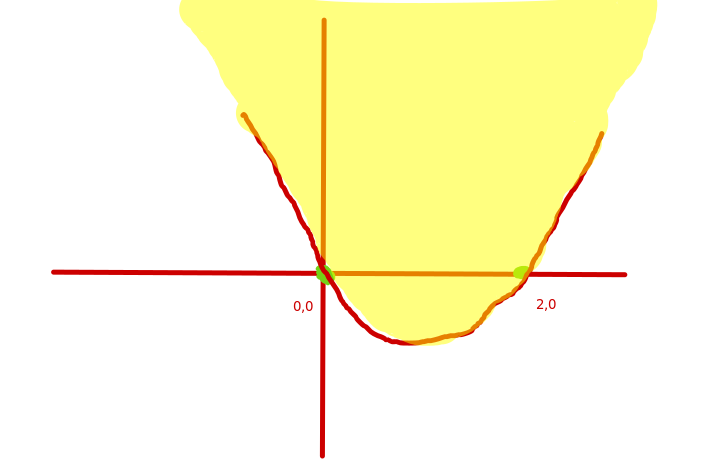
\includegraphics[scale = 0.5]{q11}
\end{figure}

\subsubsection{Item 2}

\[C_{k} = \lbrace (x,y) \in \mathds{R}^{2} / \sqrt{y-x^{2}+2x} = k \rbrace\]
\[C_{0} \longrightarrow \sqrt{y-x^{2}+2x} = 0 \longrightarrow y-x^{2}+2x = 0 \longrightarrow y = x^{2}-2x \longrightarrow y = x(x-2)\]
\[C_{1} \longrightarrow \sqrt{y-x^{2}+2x} = 1 \longrightarrow y-x^{2}+2x = 1 \longrightarrow y = x^{2}-2x+1 \longrightarrow y = (x-1)^{2}\]
\[C_{2} \longrightarrow  y = x^{2}-2x+4 \longrightarrow y = (x-1)^{2}+3\]
\[C_{3} \longrightarrow  y = x^{2}-2x+9 \longrightarrow y = (x-1)^{2}+8\]
\[\vdots\]
\begin{figure}[h!]
	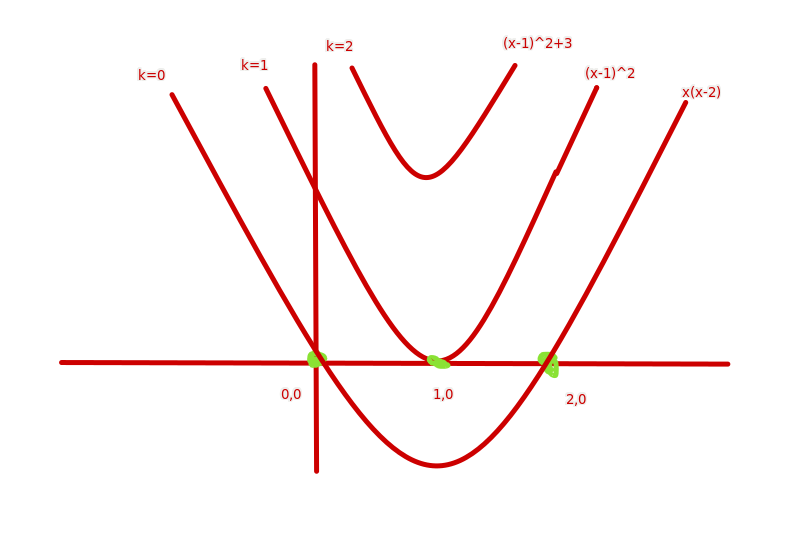
\includegraphics[scale = 0.5]{q12}
\end{figure}\\\\\\

\subsection{Questão 2}
\subsubsection{Item 1}

\[\dfrac{y^{3}}{y^{2}+x^{2}} = \dfrac{y^{2}}{y^{2}+x^{2}} \cdot y\]
\[\dfrac{y^{2}}{y^{2}+x^{2}} \text{ é limitado pois } y^{2} \leq y^{2}+x^{2} \text{ já que todo número real ao quadrado é positivo}\]
\[\text{além de } \lim_{(x,y) \rightarrow (0,0)} y = 0\]
\[\text{portanto } \lim_{(x,y) \rightarrow (0,0)} \dfrac{y^{3}}{y^{2}+x^{2}} = 0\]

\subsubsection{Item 2}

\[\text{Avalia-se o limite em duas retas: } x = 0 \text{ e } y = 0\]
\[x = 0 \longrightarrow \lim_{(x,y) \rightarrow (0,0)} \dfrac{|y|}{|y|} = \lim_{(x,y) \rightarrow (0,0)} 1 = 1\]
\[y = 0 \longrightarrow \lim_{(x,y) \rightarrow (0,0)} \dfrac{0}{|x|} = \lim_{(x,y) \rightarrow (0,0)} 0 = 0\]
\[\text{Os limites laterais de um mesmo ponto da função tem valores diferentes, portanto o limite não existe}\]

\subsection{Questão 3}
\subsubsection{Item 1}

\[\dfrac{\partial f}{\partial x} = \dfrac{(x^{2}+y^{2}) \cdot y^{3} - xy^{3} \cdot 2x}{(x^{2}+y^{2})^{2}} = \dfrac{x^{2}y^{3} + y^{5} - 2x^{2}y^{3}}{(x^{2}+y^{2})^{2}} = \dfrac{y^{5} - x^{2}y^{3}}{(x^{2}+y^{2})^{2}} = \dfrac{y^{3}(y^{2}-x^{2})}{(x^{2}+y^{2})^{2}}\]
\[\dfrac{\partial f}{\partial y} = \dfrac{(x^{2}+y^{2}) \cdot 3xy^{2} - xy^{3} \cdot 2y}{(x^{2}+y^{2})^{2}} = \dfrac{3x^{3}y^{2} + 3xy^{4} - 2xy^{4}}{(x^{2}+y^{2})^{2}} = \dfrac{3x^{3}y^{2} + xy^{4}}{(x^{2}+y^{2})^{2}} = \dfrac{xy^{2} (3x^{2}+y^{2})}{(x^{2}+y^{2})^{2}}\]

\subsubsection{Item 2}

\[\dfrac{\partial f}{\partial x}(a,b) := \lim_{t \rightarrow 0} \dfrac{f(a+t,b)-f(0,0)}{t}\]
\[\dfrac{\partial f}{\partial y}(a,b) := \lim_{t \rightarrow 0} \dfrac{f(a,b+t)-f(0,0)}{t}\]
\[\dfrac{\partial f}{\partial x}(0,0) = \lim_{t \rightarrow 0} \dfrac{f(t,0)-f(0,0)}{t} = \lim_{t \rightarrow 0} \dfrac{\dfrac{t \cdot 0}{t^{2}+0}-0}{t} = \lim_{t \rightarrow 0} \dfrac{0}{t} = \lim_{t \rightarrow 0} 0 = 0\]
\[\dfrac{\partial f}{\partial y}(0,0) = \lim_{t \rightarrow 0} \dfrac{f(0,t)-f(0,0)}{t} = \lim_{t \rightarrow 0} \dfrac{\dfrac{0 \cdot t^{3}}{0+t^{2}}-0}{t} = \lim_{t \rightarrow 0} \dfrac{0}{t} = \lim_{t \rightarrow 0} 0 = 0\]

\subsubsection{Item 3}

\[\text{A função f é diferenciável no ponto (0,0) se o limite } \dfrac{xy^{3}}{x^{2}+y^{2}} \text{ existir}\]
\[\dfrac{xy^{3}}{x^{2}+y^{2}} = \dfrac{y^{2}}{x^{2}+y^{2}} \cdot xy\]
\[\dfrac{y^{2}}{x^{2}+y^{2}} \text{ é limitado, como visto na questão 2}\]
\[\text{além de } \lim_{(x,y) \rightarrow (0,0)} xy = 0\]
\[\text{portanto } \lim_{(x,y) \rightarrow (0,0)} \dfrac{y^{3}}{y^{2}+x^{2}} = 0\]
\[\text{O limite existe, e então f é diferenciável em (0,0)}\]

\subsection{Questão 4}
\subsubsection{Item 1}

\[\dfrac{\partial f}{\partial x} = \dfrac{1}{x+\sqrt{x^{2}+y^{2}}} \left( 1 + \dfrac{1}{2\sqrt{x^{2}+y^{2}}} \right) 2x = \dfrac{1}{x+\sqrt{x^{2}+y^{2}}} \left(1 + \dfrac{x}{\sqrt{x^{2}+y^{2}}}\right) =\]
\[= \dfrac{1}{x+\sqrt{x^{2}+y^{2}}} \left( \dfrac{x+\sqrt{x^{2}+y^{2}}}{\sqrt{x^{2}+y^{2}}} \right) = \dfrac{1}{\sqrt{x^{2}+y^{2}}}\]
\[\dfrac{\partial}{\partial y} \left( \dfrac{1}{\sqrt{x^{2}+y^{2}}} \right) = \dfrac{-1}{2\sqrt{x^{2}+y^{2}}} \cdot (x^{2}+y^{2}) \cdot 2y = \dfrac{-y}{(x^{2}+y^{2})\sqrt{x^{2}+y^{2}}}\]
\[\dfrac{\partial f}{\partial y} = \dfrac{1}{x+\sqrt{x^{2}+y^{2}}} \left( \dfrac{1}{2\sqrt{x^{2}+y^{2}}} \right) \cdot 2y = \dfrac{1}{x+\sqrt{x^{2}+y^{2}}} \left( \dfrac{x-\sqrt{x^{2}+y^{2}}}{x-\sqrt{x^{2}+y^{2}}} \right) \left( \dfrac{y}{\sqrt{x^{2}+y^{2}}} \right)\]
\[\dfrac{x-\sqrt{x^{2}+y^{2}}}{y^{2}} \left( \dfrac{y}{\sqrt{x^{2}+y^{2}}} \right) = \dfrac{-x+\sqrt{x^{2}+y^{2}}}{y\sqrt{x^{2}+y^{2}}} = \dfrac{-x}{y\sqrt{x^{2}+y^{2}}} + \dfrac{1}{y}\]
\[\dfrac{\partial}{\partial x}\left( \dfrac{-x}{y\sqrt{x^{2}+y^{2}}} + \dfrac{1}{y} \right) = \dfrac{-y\sqrt{x^{2}+y^{2}} + \dfrac{x^{2}y}{\sqrt{x^{2}+y^{2}}} }{y^{2}(x^{2}+y^{2})} \cdot \left( \dfrac{\sqrt{x^{2}+y^{2}}}{\sqrt{x^{2}+y^{2}}} \right) =\]
\[= \dfrac{-y(x^{2}+y^{2}) + x^{2}y}{y^{2}(x^{2}+y^{2})\sqrt{x^{2}+y^{2}}} = \dfrac{y(x^{2}-(x^{2}+y^{2}))}{y^{2}(x^{2}+y^{2})\sqrt{x^{2}+y^{2}}} = \dfrac{-y^{2}}{y(x^{2}+y^{2})\sqrt{x^{2}+y^{2}}} = \dfrac{-y}{(x^{2}+y^{2})\sqrt{x^{2}+y^{2}}}\]
\[\dfrac{\partial^{2}f}{\partial x\partial y} = \dfrac{\partial^{2}f}{\partial y\partial x}\]

\subsubsection{Item 2}

\[\text{Equação do plano: } \mathds{P}: z-f(a,b) = \dfrac{\partial f}{\partial x}(a,b)(x-a) + \dfrac{\partial f}{\partial y}(a,b)(y-b)\]
\[\dfrac{\partial f}{\partial x} (0,1) = \dfrac{1}{\sqrt{0+1}} = 1\]
\[\dfrac{\partial f}{\partial y} (0,1) = \dfrac{1}{0+1+0\sqrt{0+1}} = 1\]
\[f(0,1) = \ln(0+\sqrt{0+1}) = \ln1 = 0\]
\[\mathds{P}: z-0 = 1(x-0) + 1(y-1)\]
\[\mathds{P}: z = x+y-1\]
\[\mathds{P}: x+y-z = 1\]

\subsubsection{Item 3}

\[\overrightarrow{u} \text{ é unitário pois } \left( \dfrac{3}{5} \right)^{2} + \left( -\dfrac{4}{5} \right)^{2} = \dfrac{9}{25} + \dfrac{16}{25} = 1\]
\[\text{Portanto: } \dfrac{\partial f}{\partial \overrightarrow{u}} = \bigtriangledown f(a,b) \cdot \overrightarrow{u} =  \dfrac{\partial f}{\partial x}(a,b)u_{1} + \dfrac{\partial f}{\partial y}(a,b)u_{2}\]
\[1 \cdot \dfrac{3}{5} + 1 \cdot \left( -\dfrac{4}{5} \right) = -\dfrac{1}{5}\]

\end{document}